% This is samplepaper.tex, a sample chapter demonstrating the
% LLNCS macro package for Springer Computer Science proceedings;
% Version 2.21 of 2022/01/12
%
\documentclass[runningheads]{llncs}
%
\usepackage[T1]{fontenc}
% T1 fonts will be used to generate the final print and online PDFs,
% so please use T1 fonts in your manuscript whenever possible.
% Other font encondings may result in incorrect characters.
%
\usepackage{graphicx}
% Used for displaying a sample figure. If possible, figure files should
% be included in EPS format.
%
% If you use the hyperref package, please uncomment the following two lines
% to display URLs in blue roman font according to Springer's eBook style:
%\usepackage{color}
%\renewcommand\UrlFont{\color{blue}\rmfamily}
%\urlstyle{rm}
%
\begin{document}
%
\title{CS-2704 Final Project Report}
%
%\titlerunning{Abbreviated paper title}
% If the paper title is too long for the running head, you can set
% an abbreviated paper title here
%
\author{Jamie Greening\inst{1}\orcidID{3543841}}
%
\authorrunning{J. Greening}
% First names are abbreviated in the running head.
% If there are more than two authors, 'et al.' is used.
%
\institute{University of New Brunswick Saint John, Saint John NB E2L 4L5, CAN
\email{jgreenin@unb.ca}}
%
\maketitle              % typeset the header of the contribution
%
%\begin{abstract}
%The abstract should briefly summarize the contents of the paper in
%150--250 words.

%\keywords{First keyword  \and Second keyword \and Another keyword.}
%\end{abstract}
%
%
%
\section{Introduction and Background}
Broadly, price increases or decreases on certain goods can affect consumer behaviour and purchasing decisions, as demonstrated by recent rises in inflation: ``Demand in some categories, such as meat, is falling as consumers adjust their shopping habits to make their grocery spending go as far as possible.'' \cite{ref_art1}. Some goods may respond differently than others: gasoline, for example, is cited as an inelastic good: ``In effect, gasoline prices could be an ``inelastic'' good, economic parlance for a product or service for which demand does not change much in response to higher prices, Tal said.'' \cite{ref_art2}. Others disagree: in an article published for the Federal Reverse Bank of Dallas, Lutz Kilian and Xiaoqing Zhou examine gas demand responding more to price changes than previously considered: ``The interesting economic question is why the fuel consumption responses are so strong. Clearly, in the short run, consumers won’t choose to replace their vehicle with a more fuel-efficient one. There are other margins of adjustment, however. For example, consumers may reduce their discretionary driving.''\cite{ref_art3}. If drivers may reduce discretionary driving as gas prices rise, would this mean that road collisions would decrease as well, implying an association between the two?
\section{Hypothesis}
I hypothesize that there will be some association between gas prices rising and road collisions decreasing, assuming that gas price fluctuations have some effect on demand for gasoline and therefore driving habits and choices. With people choosing to be on the road less (either by cutting down on non-essential driving or optimizing the time spent driving), fewer collisions should occur ideally. When gas prices go down, people might be motivated to leisure drive more and this could lead to more collisions.

That being said, other factors could influence collisions. Education programs that emphasize safe driving could have an impact on lowering collisions, as could efforts to reduce reckless driving and enforcing driving laws. Even if an association is found between gas prices and road collisions, this might not be telling the full story.

The two datasets I will be using are:
\begin{itemize}
    \item National Collision data, from the National Collision Database \cite{ref_url1}
    \item Monthly average retail prices for gasoline and fuel oil, by geography \cite{ref_url2}
\end{itemize}

Both datasets have also been cleaned and summarized for easier analysis. This includes:
\begin{itemize}
    \item Averaging monthly fuel prices for cities included in the gas dataset, to create an approximate national average for 1999-2005
    \item Removing columns and rows irrelevant to the analysis (the collision data had a significant amount of extra data included)
    \item Setting date formats to be equal so both series (gas prices and number of collisions, by month) could be charted in one figure
\end{itemize}
\section{Analysis and Implication}
As a start, average monthly gas prices and number of collisions per month were both charted using a line plot as can be seen in figures \ref{fig:collision-label} and \ref{fig:gas-label}.
\begin{figure}
    \centering
    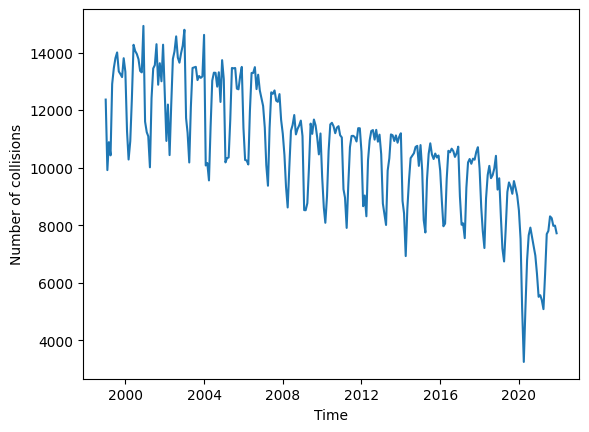
\includegraphics[scale=0.75]{Collision_Chart.png}
    \caption{Number of collisions over time, by month}
    \label{fig:collision-label}
\end{figure}

\begin{figure}
    \centering
    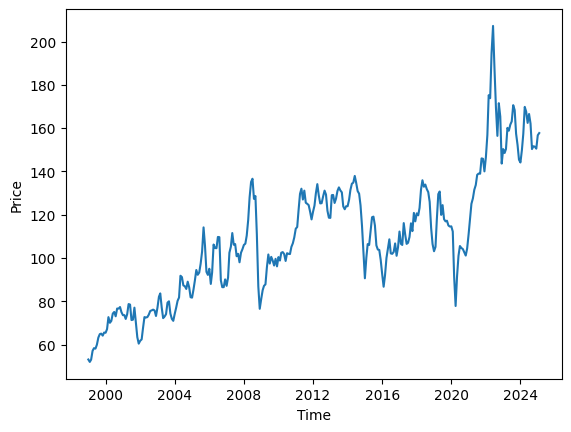
\includegraphics[scale=0.75]{Gas_Chart.png}   
    \caption{Average gas prices over time, by month}
    \label{fig:gas-label}
\end{figure}

Next, both variables were charted together in figure \ref{fig:both-label} and \ref{fig:scatter-label} to determine if there may potentially be a relationship between the two.

\begin{figure}
    \centering
    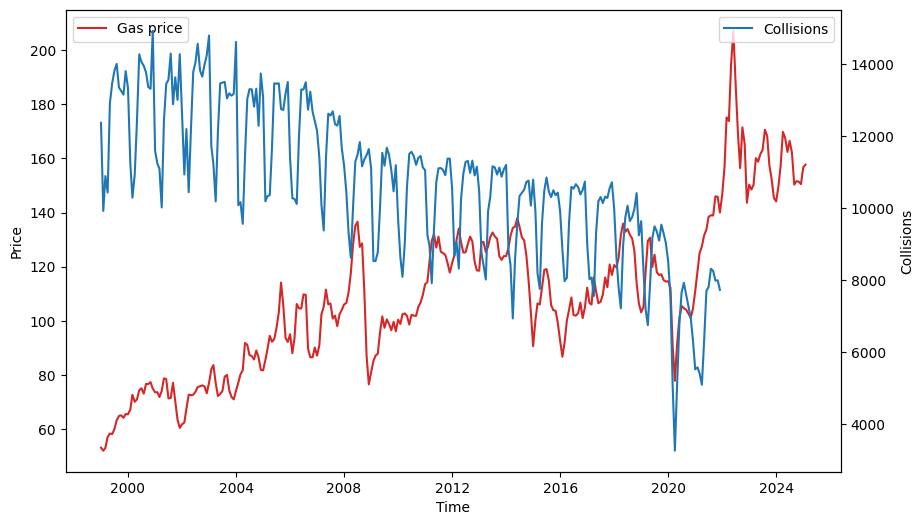
\includegraphics[scale=0.45]{Both_Chart.png}   
    \caption{Average gas prices and number of collisions over time, by month}
    \label{fig:both-label}
\end{figure}

\begin{figure}
    \centering
    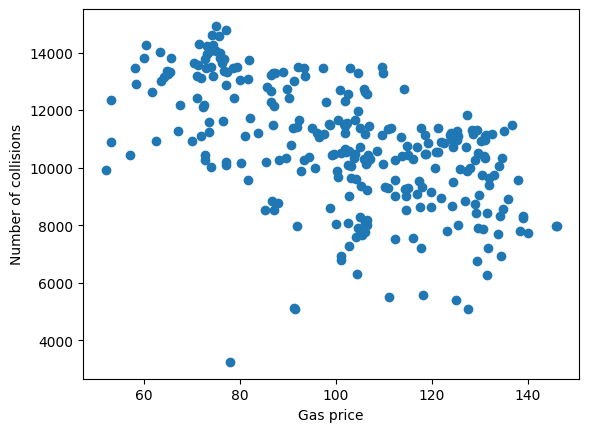
\includegraphics[scale=0.75]{Scatter.png}   
    \caption{Average gas prices and number of collisions by month, in a scatterplot}
    \label{fig:scatter-label}
\end{figure}

Over the last two decades, it appears that monthly collisions have trended down as gas prices have gone up. Unfortunately, collision data is only available up until around 2022, so the potential effect of the large spike in gas prices after that same period on collisions cannot be determined.

Using Linear Regression, a model was created and tested using average gas prices by month as the predictor variable and number of collisions by month as the outcome variable. The model was tested with a variety of test sizes, as can be seen below in figures \ref{fig:r2-label} and \ref{fig:accuracy-label}. From this, it appears that our linear regression model was not particularly accurate when it came to predicting the number of collisions based on gas prices as input. With a test size of 0.3 and 0.45, the \(R^2\) score gets close to 0 (indicating how a baseline model would do) but never reaches it. Notably, the \(R^2\) appears to vary greatly - when the test was ran at 5:02 PM on April 16 2025, the \(R^2\) for one test size appears to surpass the performance of a baseline model as can be seen in figure \ref{fig:r2_later_label}. This would seem to indicate that gas prices are not particularly predictive when it comes to the number of collisions per month.

\begin{figure}
    \centering
    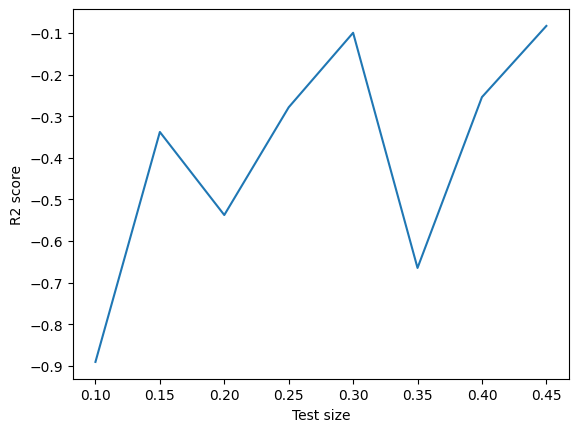
\includegraphics[scale=0.75]{R2_CHART.png}   
    \caption{\(R^2\) score by test size, ran at 4:52 PM on April 16 2025}
    \label{fig:r2-label}
\end{figure}

\begin{figure}
    \centering
    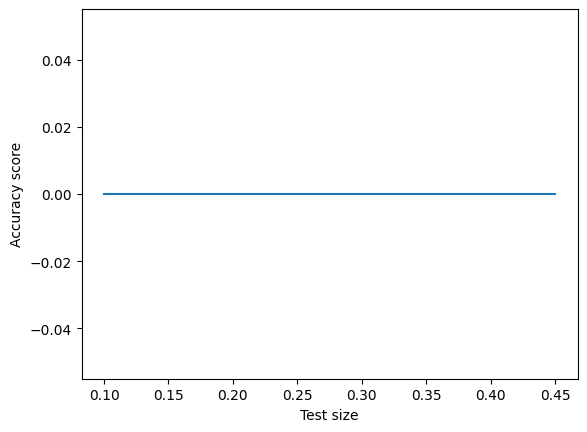
\includegraphics[scale=0.75]{Accuracy_Chart.png}   
    \caption{Accuracy score by test size}
    \label{fig:accuracy-label}
\end{figure}

\begin{figure}
    \centering
    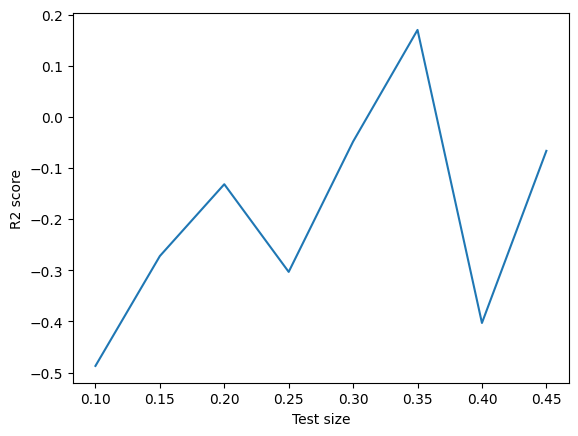
\includegraphics[scale=0.75]{R2_502pm.png}   
    \caption{\(R^2\) score by test size, ran at 5:02 PM on April 16 2025}
    \label{fig:r2_later_label}
\end{figure}

\section{Conclusion}
Based on the results of the analysis done, it does not appear there is a particularly strong or predictive relationship between gas prices and number of collisions. While there was some variance in \(R^2\) when tests were repeatedly done, it appears the Linear Regression model at its best will only perform marginally better than a baseline model. Notably, per figure \ref{fig:accuracy-label}, it does not appear the model was ever accurate (per sklearn's accuracy\_score method). While it could appear there is a relationship between the two based on figures \ref{fig:both-label} and \ref{fig:scatter-label}, there also appears to be a lot of variance - notably, there are periodic increases and declines in collisions within every year. Further research and experimentation could be done with the additional data that the National Collision Database\cite{ref_url1} can provide. As an example, could gas prices have more of a relationship with the severity of a crash (lower gas prices, potentially more risky driving and speeding, increase in fatalities)? 
%
% ---- Bibliography ----
%
% BibTeX users should specify bibliography style 'splncs04'.
% References will then be sorted and formatted in the correct style.
%
% \bibliographystyle{splncs04}
% \bibliography{mybibliography}
%
\begin{thebibliography}{8}
\bibitem{ref_url1}
Transport Canada: National Collision Database Online. Online. \url{https://wwwapps2.tc.gc.ca/Saf-Sec-Sur/7/NCDB-BNDC/p.aspx?l=en}, last accessed 2025-03-28

\bibitem{ref_url2}
Statistics Canada: Monthly average retail prices for gasoline and fuel oil, by geography. Online. \url{https://www150.statcan.gc.ca/t1/tbl1/en/tv.action?pid=1810000101}, last accessed 2025-03-28

\bibitem{ref_art1}
CBC: Prices for many foods coming down, but inflation has left a legacy. Kevin Yarr. Online. \url{https://www.cbc.ca/1.7192916}, last accessed 2025-04-16

\bibitem{ref_art2}
CBC: Higher gas prices to bite Canadian drivers: CIBC. Online. \url{https://www.cbc.ca/news/business/higher-gas-prices-to-bite-canadian-drivers-cibc-1.977899}, last accessed 2025-04-16

\bibitem{ref_art3}
Federal Reserve Bank of Dallas: Gasoline demand more responsive to price changes than economists once thought. Lutz Kilian and Xiaoqing Zhou. Online. \url{https://www.dallasfed.org/research/economics/2020/0616}, last accessed 2025-04-16

\end{thebibliography}
\end{document}
